%%%%%%
%
% $Autor: Wings $
% $Datum: 2020-01-18 11:15:45Z $
% $Pfad: WuSt/Skript/Produktspezifikation/powerpoint/ImageProcessing.tex $
% $Version: 4620 $
%
%%%%%%

\chapter{Neural Networks}

While computers are superior to humans in many areas, there are nevertheless tasks that a human can
intuitively due to their intelligence and ability to learn, while transferring these abilities to the 
transferring these abilities to the computer is a great challenge. A popular approach to the development of 
artificial intelligence lies in artificial neural networks. These are 
information-processing systems whose structure and mode of operation are modelled on the nervous system, especially the 
and especially the brains of animals and humans.

Neuronal networks consist - according to their name - of neurons, which are interconnected 
and influence each other. Like their biological counterparts, the modelled neurons can, if sufficiently 
sufficient stimulation by one or more input signals. The biological 
neuron can be compared to a capacitor that is charged by small electrical voltage pulses from other neurons. 
from other neurons. If the voltage thus reached exceeds a threshold value, 
the neuron itself transmits a voltage pulse to connected neurons. This principle is used in 
artificial neural networks by mathematical models. Figure \ref{NNBio} shows 
the first stage of abstraction from biological neural networks to mathematical models. 
\cite{Ertel:2016}

\begin{figure}[H]
	\begin{center}
		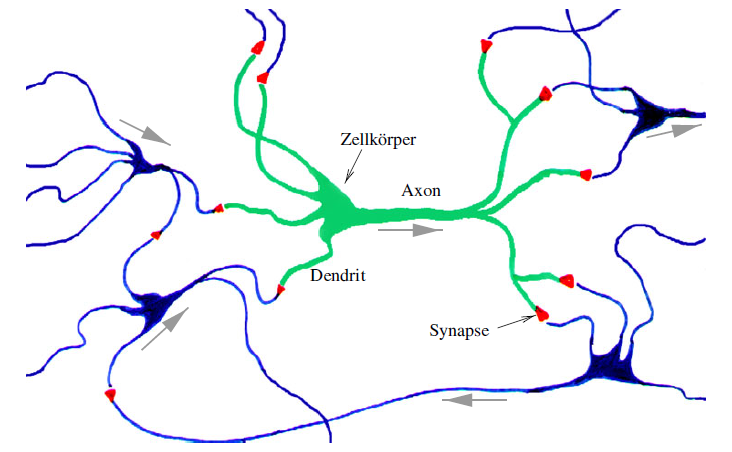
\includegraphics[width=0.49\textwidth]{NeuralNetwork/NeuronBio}
		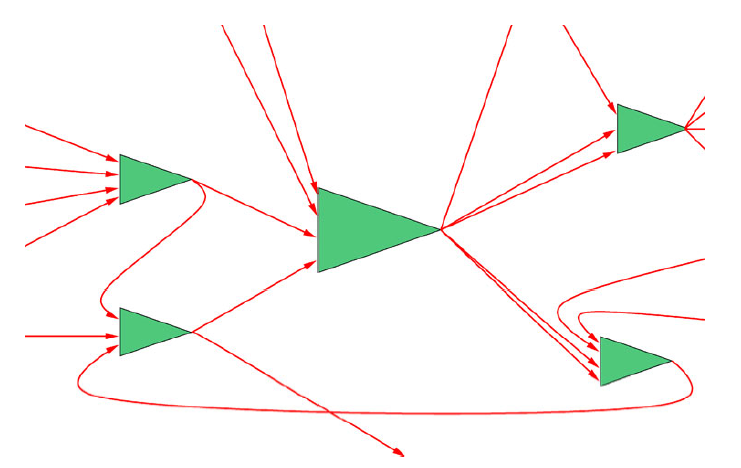
\includegraphics[width=0.49\textwidth]{NeuralNetwork/NeuronAbstrakt}
		\caption{Biological (left) and abstracted (right) model of neural networks. Source:\cite{Ertel:2016}} 
		\label{NNBio}
	\end{center}
\end{figure}

In 1958, Frank Rosenblatt presented the simplest form of a neural network. This model, presented as a
as a single-layer perceptron, contains a layer of input neurons, each connected to an output neuron.
all connected to an output neuron. \cite{Dorn:2018} If several neurons are connected in layers in 
connected in series, we are talking about the multilayer perceptron. The output
neuron acts as an input signal for the following neuron, until a final output is
final output takes place at the output layer.

\section{Mathematical Modelling} 

The birth of neural network AI can be seen in the 1943 publication \glqq A logical calculus of the ideas immanent in nervous activity\grqq \cite{McCulloch:1943} by McCulloch and Pitts. In their description, neurons can have either the output value 0 for inactivity or 1 for activity. This is referred to as binary neural networks. (Sometimes the activity level -1 for inactivity is also used, cf. \cite{Ertel:2016}). With McCulloch and Pitts, the input values for a neuron are added together and this is set to activity level 1 if this sum exceeds a predefined threshold $\theta$. One therefore also speaks of \glqq threshold elements\grqq \cite{Kruse:2015}, a representation of how this works, taking into account different weights $w_1$ and $w_2$, can be seen in Figure \ref{threshold element}. Several neurons are connected in layers to form networks in order to be able to map complex relationships. As will be described in the following, different weights (section \ref{weights}), as well as activation and output functions (section \ref{activation and output function}) with continuous (instead of binary) output values and different architectures play a role in more complex neural networks. With the mathematical modelling of the neuron, however, McCulloch and Pitts laid the foundation for the further development of neural networks, although the computer technology of the time was not yet sufficiently powerful for the simulation of simple brain structures. \cite{Ertel:2016}

\begin{figure}[H]
	\begin{center}
		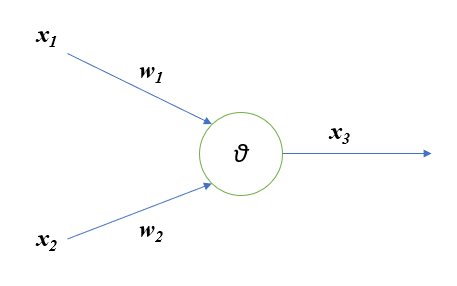
\includegraphics[width=0.6\textwidth]{NeuralNetwork/Schwellenwertelement}
		\caption{Representation of a neuron as a simple threshold element} 
		\label{Schwellenwertelement}
	\end{center}
\end{figure}

\subsection{Weights} \label{Gewichte}

In order to be able to map different relationships between the activations of the neurons, the information flows between the neurons are weighted differently. In addition, constant input values can provide a neuron-specific bias, the weighting of which may also need to be determined. \cite{Moeser:2018} In the representation of the network as a directed graph, the weights are usually specified at the edges.  Mathematically, the representation as a matrix is common. An example of the graph representation and the equivalent weight matrix can be seen in Figure \ref{weightmatrix}. The weights are often named by convention with first the index of the neuron receiving the signal as input and then the index of the sending neuron.

\begin{figure}[H]
	\begin{center}
		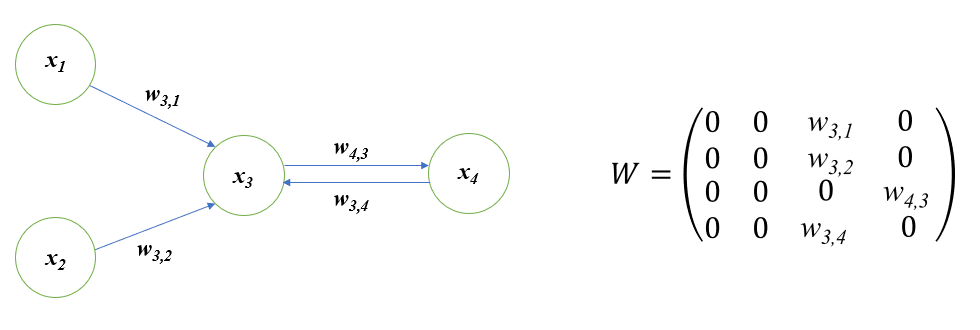
\includegraphics[width=1\textwidth]{NeuralNetwork/Gewichtsmatrix}
		\caption{Graph with weighted edges and equivalent weight matrix} 
		\label{Gewichtsmatrix}
	\end{center}
\end{figure}

At the beginning, the weights are set to random values. Usually values between -1 and 1 are chosen, although the values resulting from the training can also lie outside this interval. \cite{Moeser:2018} For certain(!) training methods, initialisation with zeros is also conceivable. \cite{Kononenko:2007}

\subsection{Bias}

Bias is the neuron-specific bias that can be interpreted as an additional input with a constant value. The bias value can be modelled both explicitly or as a weighting of an additional constant input value and can strengthen or weaken the result of a neuron. \cite{Ziegler:2015}

\subsection{activation and output function} \label{activation and output function} 

Which value a neuron passes on depends on the incoming signals, their weighting, the activation function and the output function. From the incoming output signals of the connected neurons (and possibly the feedback of the own output signal of the considered neuron itself), the activation function $f$ calculates the activity level of the neuron, taking into account the weighting of the signals. \cite{Kruse:2015} The output of the neuron $x_i$ is calculated from the $w_{ij}$ weighted incoming signals of the $n$ neurons $x_j$ with $j = 1...n$.

\begin{center}
$x_i = f(\sum \limits_{j=1}^n w_{ij} x_j)$
\end{center}

In the simplest case, the activation function is linear, then the signals are added weighted and possibly scaled with a constant factor. More complex, non-linear relationships can only be modelled using linear activation functions in multi-layer networks.\cite{Kononenko:2007} Non-linear functions facilitate generalisation and adaptation to diverse data and are therefore widely used. \cite{Gupta:2020b}

The output value of the neuron is then determined from the activity level of the neuron determined in this way, with the help of the output function. In most cases, the identity is used as the output function \cite{Beck.2018}, so that often only the activation function is addressed and the output function is neglected.

\subsubsection{ReLu Function}

The Rectified Linear Unit function is considered the most commonly used activation function. It is defined as $R(z)=max(0,z)$, i.e. all negative values become zero and all values above zero remain unchanged. However, this can also lead to problems, as negative activations are ignored and neurons are deactivated. This is what the Leaky ReLu function is designed to correct, using a low slope <1 in the negative range (see figure \ref{ReLu}). Both functions and their derivatives are monotonic. This is important so that the activation cannot decrease with increasing input values. \cite{Gupta:2020b}\cite{AIUnitedRedaktion.20.12.2018}

\begin{figure}[H]
	\begin{center}
		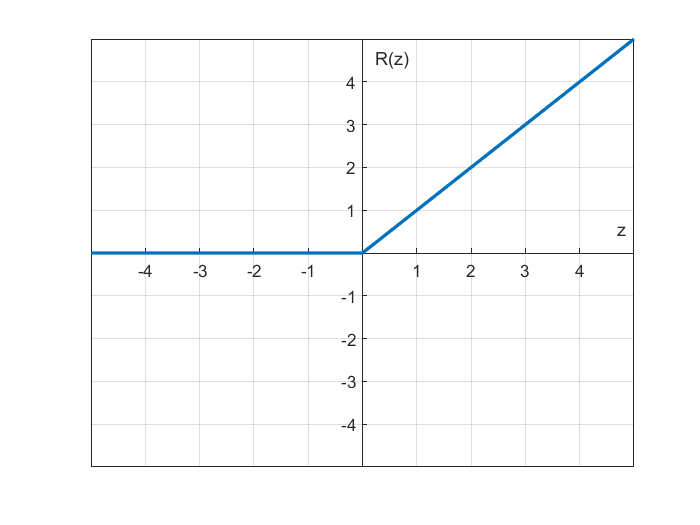
\includegraphics[width=0.49\textwidth]{NeuralNetwork/ReLu}
		\includegraphics[width=0.49\textwidth]{NeuralNetwork/LeakyReLu}
		\caption{ReLu function (left) and Leaky ReLu} 
		\label{ReLu}
	\end{center}
\end{figure}

\subsubsection{Sigmoid Function} 

The sigmoid function transforms the input values into the range [0,1], see figure \ref{Sigmoid}. The function for this is $S(z)=\frac{1}{1+e^{-z}}$. Due to the range of values, the function is well suited for the representation of probabilities. It is always positive, so that the output cannot have a weakening influence on the subsequent neurons. The function is differentiable and monotonic, but its derivative is not monotonic. \cite{Gupta:2020b}\cite{AIUnitedRedaktion.20.12.2018}

\begin{figure}[H]
	\begin{center}
		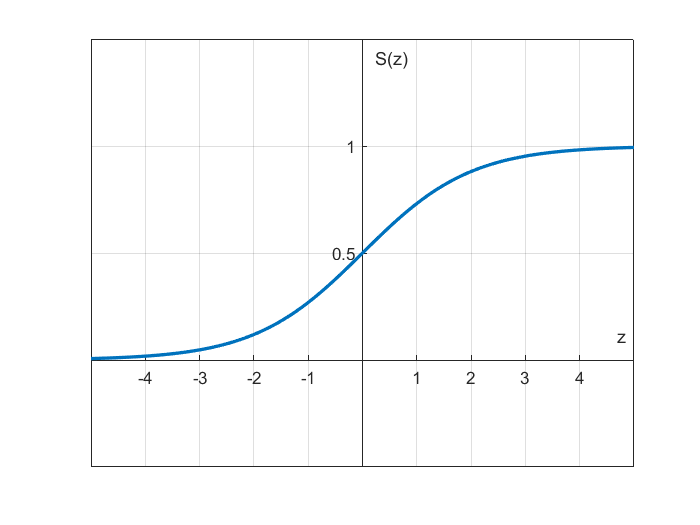
\includegraphics[width=0.6\textwidth]{NeuralNetwork/Sigmoid}
		\caption{Sigmoid function} 
		\label{Sigmoid}
	\end{center}
\end{figure}

\subsubsection{Softmax Function}

The softmax function is often described as a superposition of several sigmoid functions. It is mainly used in the output layer to reflect the probabilities for the different categories. The mathematical expression for the softmax function is \cite{Gupta:2020b}:

\begin{center}
$\sigma(z)_j = \frac{e^{z_j}}{\sum\nolimits_{k=1}^K e^{z_k}}$
\end{center}

%Die Softmax-Funktion ist eine Aktivierungsfunktion zur Identifizierung verschiedener Klassen. Es wird die Wahrscheinlichkeitsverteilung jedes Ergebnisses berechnet. Dabei ist die
%	Summe aller möglichen Wahrscheinlichkeiten immer 1. Die einzelnen Wahrscheinlichkeitsbereiche befinden 
%	sich zwischen $0$ und $1$. Die Ausgabe der Softmax-Funktion ist das Verhältnis
%	des Exponentials des Eingabewerts und der Summe der Exponentialwerte. Typischerweise
%	befindet sich die Softmax-Funktion im Output-Layer, kann aber auch in verschiedenen
%	Schichten verwendet werden. \cite{Polamuri:2017}

\subsection{tanh Function}%neu

The tangent hyperbolic function is a non-linear function in the value range from $-1$ to $1$. It is similar to the sigmoid function with the major difference of point symmetry at the origin. The function is defined as:

\begin{center}
  $\tanh(z) = \frac{2}{1 + e^{-2z}} -1$
\end{center}

The negative inputs are strongly negative and the zero inputs are close to the zero point of the diagram. Negative outputs can occur, which can also negatively affect the weighted sum of a neuron of the following layer. This function is particularly well suited to the differentiation of two classes. The function is differentiable, monotonic and the derivative is non-monotonic. \cite{Gupta:2020b} The figure~\ref{NNTanh} shows the function tangent hyperbolicus in the definition range from $-6$ to $6$.

\begin{figure}[H]
	\begin{center}
	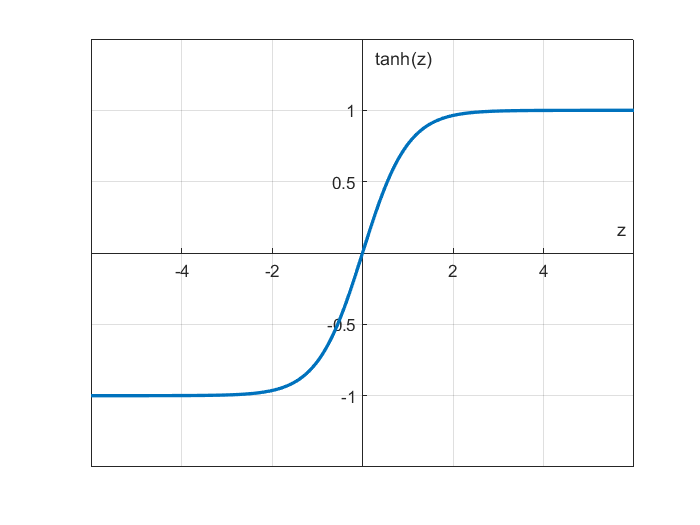
\includegraphics[width=0.6\textwidth]{NeuralNetwork/Tanh}
	\caption{Funktion Tangens Hyperbolicus}\label{NNTanh}
	\end{center}
\end{figure}

	
	

\section{Training}%mögliche Ergänzung: Hebb-Regel (unüberwachtes Lernen)

The great strength of neural networks lies in their ability to learn. In neural networks, the learning process consists of adapting the weights with the aim of outputting the desired output value(s) in the output layer in the case of corresponding input signals in the input layer. For this purpose, the weights are first initialised randomly and then adjusted according to the learning rules.


\subsection{Propagation}

Propagation refers to the process in which information is sent via the input layer into the network and passes through it to the output layer. If the information only moves from the input to the output layer, it is referred to as a forward network or forward propagation. At the beginning, the input is copied into the input layer and then forwarded to the first hidden layer. What information this layer passes on to the next depends on the weights and the activation functions. Finally, the output can be read from the output layer. \cite{Kriesel:2008}


\subsection{error}

Error is the deviation between the actual network output and the desired network output after the input data has been propagated through the entire neural network. \cite{Kriesel:2008}


\subsection{Delta Rule} 
The basis of the learning process is the delta rule. For each input data point in the learning phase, the difference between the actual and expected (correct) output is determined. Then the weights are changed so that the error becomes smaller. To determine the direction in which the weights must be changed, the derivative of the error function is used (gradient descent). The strength of the adjustment is determined by the learning rate. This process is repeated iteratively until the termination criterion, e.g. a sufficiently small error, is met.\cite{Kononenko:2007}

\begin{center}
$\Delta w_{ij} = \varepsilon  (x_i - l_i)  f'(\sum_{j} w_{ij} x_j) $
\end{center}

This rule can only be applied directly to the weights between the output layer and the layer before it. For the layers before it, the error must be propagated backwards through the network, since the desired outputs for the hidden networks are not given. \cite{Kruse:2015} 

\subsection{Error Backpropagation}. 

In the backpropagation procedure, the change in the values of the hidden neurons is recursively calculated from the change in the neurons in the higher layer. For this, the network output must first be calculated (forward propagation). The error obtained is used in backward propagation to adjust the weights from layer to layer. This process is applied to all training data until the termination criterion is met. \cite{Ertel:2016}

This procedure is well established for training neural networks. Nevertheless, there are some difficulties that need to be taken into account. For example, a local minimum of the error can be found, which is not left anymore, so that the global minimum cannot be found. This problem can be mitigated by running the procedure with different starting values. \cite{Kruse:2015}

\subsection{Problem of Overfitting}

If a neural network is repeatedly trained with known data sets, the network may learn the data by heart instead of developing an abstract concept.
develop. This condition is called overfitting. For this reason, not all data should be used for training. It makes sense to withhold a validation set and a test set. \cite{Becker:2018}

	
	
\subsection{Epochs, Batches and Steps}

An epoch is a complete run of all input data, with the measurement of the error, and backpropagation to adjust the weights. For large data sets, the input data can be divided into groups of equal size, called batches. In this way, a neural network can be trained more quickly. It is important that the values within each batch are normally distributed. For example, if a data set of 2,000 images is divided into batches of 10 images each, the epoch will run through 200 steps. Alternatively, the number of steps can be specified and the batch size adjusted accordingly.\cite{Becker:2018c}

\subsection{Dropout}

Dropout disables some neurons by multiplying a defined percentage of neurons by zero during forward propagation. These neurons have
no longer have any influence on subsequent activations. Deactivation occurs on a random basis per run. If a neuron is imprinted on a feature and fails, the surrounding neurons learn to deal with this problem. This increases the generalisation of the network, it learns more abstract concepts. A disadvantage is the increase in training time, because the parameter feedback is noisy. At the end of the training, all neurons are reactivated. \cite{Becker:2018c}

\subsection{Correct Classification Rate and Loss Function}

The correct classification rate measures the ability of the network to assign data points to the correct class. This contrasts with the loss function. \cite{Chollet:2018}

Both are often documented during the training process to allow conclusions to be drawn about the training process and to identify problems such as overfitting or too few runs.

\subsection{Training Data, Validation Data and Test Set}

The training data is actively used to teach the network the features of the classifications. 	The validation data is fed to the network at the end of each epoch to test how accurately the network performs. Even if the validation set is not actively used for training, some information flows back into the network.	For this reason, a test set is used that is not related to the training of the neural network and only has the purpose of checking the theoretical accuracy of the network. \cite{Becker:2018}

\subsection{Transfer Learning}

Transfer learning means the transfer of the results of a finished neural network to a new task. 	Layers can be kept constant and only the output layer can be retrained.
or several layers can be retrained on the basis of the current training status. If several or all layers are retrained, the weights of the trained network are used as the starting point. Which strategy should be used depends on two factors:

\begin{itemize}
    \item similarity of the data
    \item size of the new data set
\end{itemize}

		
If the data sets are highly similar, transfer learning is a good way to improve a neural network. Similarities exist, for example, in a trained network for the recognition of dog breeds, which would also be suitable for the recognition of cat breeds. However, this network would be unsuitable for the recognition of different car models, as there would be too many deviations in the basic structures.	As far as the size of the data set is concerned, transfer learning may be particularly suitable for small data sets, as otherwise overfitting would quickly occur. \cite{Becker:2018}


\subsection{Weight Imprinting}

\begin{figure}[!h]
	\centering
	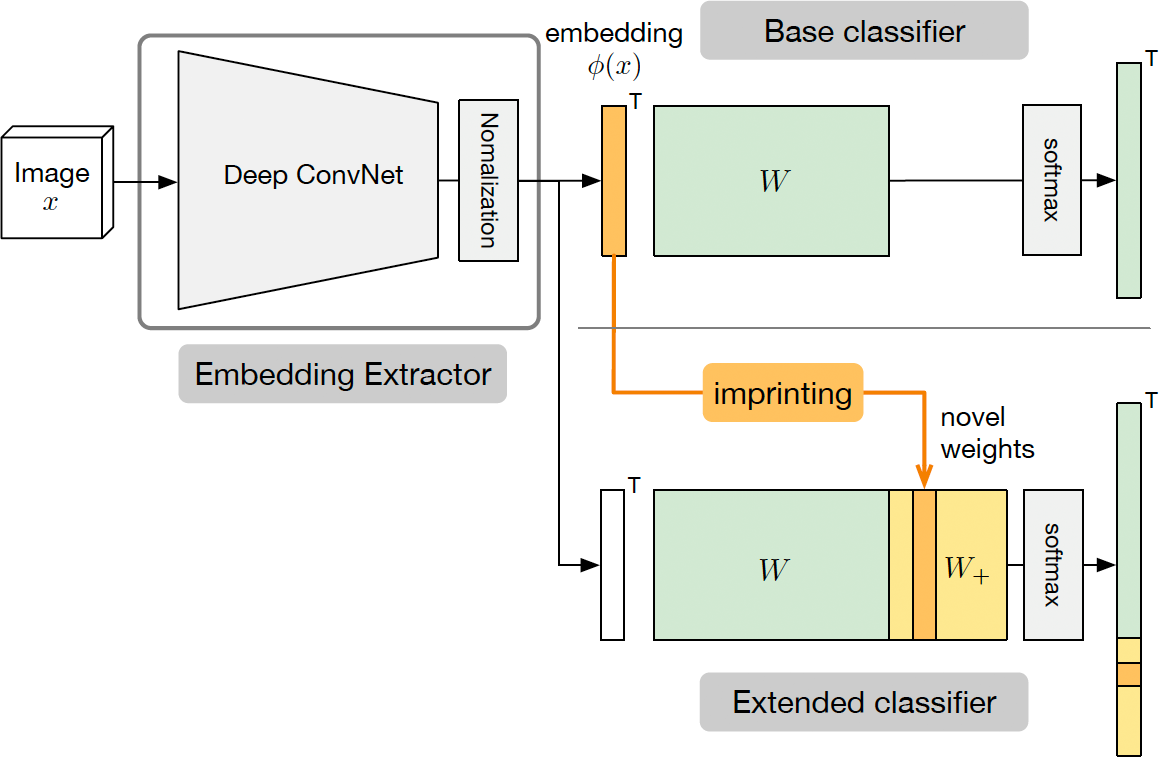
\includegraphics[scale=0.3]{/Bilder/NeuralNetwork/Weight_imprinting}
	\caption{Illustration of the weight imprinting process \cite{qi:2018}}
\end{figure}

Retraining all the weights in a model for transfer learning can be a time consuming process. In actuality, it's only the last layer of the network that decides the final classification, so only retraining the last set of weights could achieve the desired result. Weight imprinting is one such method developed by engineers at Google. Their proposed imprinting method is to directly set
the final layer weights for new classes from the embeddings
of training exemplars. Consider a single training sample
$x_{+}$ from a novel class, their method computes the embedding $\Phi(x_{+})$ and uses it to set a new column in the weight
matrix for the new class, i.e. $w_{x} = \Phi(x_{+})$. Figure 1 illustrates this idea of extending the final layer weight matrix
of a trained classifier by imprinting additional columns for
new categories.
Intuitively, one can think of the imprinting operation as
remembering the semantic embeddings of low-shot examples as the templates for new classes. \autoref{fig: EmbSpace} illustrates
the change of the decision boundaries after a new weight
column is imprinted. The underlying assumption is that test
examples from new classes are closer to the corresponding
training examples, even if only one or a few are observed,
than to instances of other classes in the embedding space.

\begin{figure}[!h]
	\label{fig: EmbSpace}
	\centering
	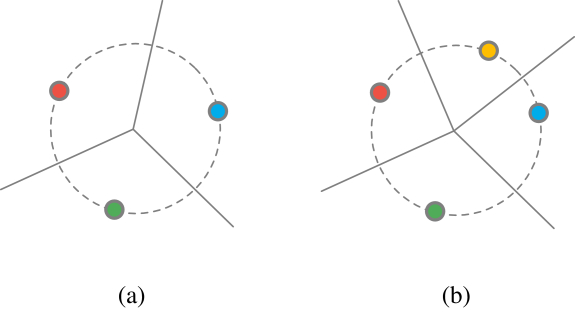
\includegraphics[scale=0.3]{/Bilder/NeuralNetwork/EmbeddingSpace}
	\caption{Illustration of imprinting in the normalized embedding
		space. (a) Before imprinting, the decision boundaries are determined by the trained weights. (b) With imprinting, the embedding
		of an example (the yellow point) from a novel class defines a new
		region. \cite{qi:2018}}
\end{figure}

\subsubsection{Average Embedding}
 If $n > 1$ examples $(x_{+}^{(i)})_{i=1}^{n}$ are
available for a new class, new weights are computed by averaging the normalized embeddings $\tilde{w}_{x} = \frac{1}{n}\sum_{i=1}^{n}\Phi(x_{+}^{(i)})$

and re-normalizing the resulting vector to unit length $w_{+} =
\frac{\tilde{w}_{+}}{||\tilde{w}_{+}||}$. In practice, the averaging operation can also
be applied to the embeddings computed from the randomly
augmented versions of the original low-shot training examples.

\subsubsection{Fine-tuning} 
Since the model architecture has the same
differentiable form as ordinary ConvNet classifiers, a finetuning step can be applied after new weights are imprinted.
The average embedding strategy assumes that examples
from each novel class have a unimodal distribution in the
embedding space. This may not hold for every novel class
since the learned embedding space could be biased towards features that are salient and discriminative among
base classes. However, fine-tuning (using backpropagation
to further optimize the network weights) should move the
embedding space towards having unimodal distribution for
the new class. \cite{qi:2018}



\section{Convolutional Neural Networks}

Complex tasks such as pattern and object recognition with high-dimensional data sets lead to convergence problems and high computation times with conventional approaches. Such tasks can be solved with deep learning algorithms. To this class belong \ac{cnn}. They can solve tasks with less preprocessing than is usual for other classification algorithms. Moreover, the filters used do not have to be designed by the user, but are learned by the network itself during training. \cite{Saha:2018}

According to \cite{Sharma:2018}, one of the first successful implementations of \ac{cnn}s was the recognition of handwritten digits in 1998, which is described in the paper \glqq Gradient-Based Learning Applied to Document Recognition\grqq \cite{LeCun:1998}. In the meantime, \ac{cnn}s have been able to prove themselves in many application areas. The typical application for \ac{cnn}s is processing data that has a known network topology. For example, they can recognise objects in images or patterns in time series. \cite{Namatevs.2017} Besides image classification, object recognition and tracking, text, speech and gesture recognition are also typical applications \cite{Gu:2018} describes. But \ac{cnn}s are also used in industry for defect detection. \cite{LopezdeLacalle:2020}

In general, \ac{cnn}s are composed of the building blocks Convolutional Layer, Pooling Layer and Fully Connected Layer, where each building block is usually used more than once. These building blocks are described below. The primary assumption is the use of \ac{cnn}s for image classification.

\subsection{Convolutional Layer}

The main component of \ac{cnn} are filters that are applied to the input data/images in the Convolutional Layer. As input, the Convolutional Layer receives an n-dimensional tensor, for example an image with three colour channels, and applies several kernels to it. By convolution of tensor and kernel, the image is filtered. The results of the convolution with the different filters are stacked so that the result is again a tensor. \cite{Michelucci:2019}

The operation of convolution between two matrices or tensors means the addition of the products of the multiplication of the corresponding elements of both matrices or tensors. Since the convolution in the Convolutional Layer usually takes place between a tensor with many entries and a small kernel, the convolution must be carried out separately for individual parts of the input tensor. Usually, one starts with the first entries at the top left and, metaphorically speaking, shifts the kernel after the first convolution relative to the input tensor by a certain number of columns and calculates the convolution again. When one has reached the right edge, the kernel is shifted in the row and the process is repeated. The value called stride indicates by how many columns and rows the kernel is shifted relative to the input tensor. In addition, an activation function is usually applied for each calculated pixel. \cite{Michelucci:2019}

In this process, a tensor with dimensions $h_1 \times w_1 \times d_1$ and kernels each with dimension $h_2 \times w_2 \times d_1$, which are stacked to form dimensions $h_2 \times w_2 \times d_2$, becomes an output tensor with dimensions $h_3 \times w_3 \times d_2$. \cite{Arunava:2018}

Here $h_3$ and $w_3$ depend on the height and width of the input tensor as well as the filters and the chosen stride, while $d_2$ is given by the number of filters.

If the size of the input tensor, the kernel and the stride do not match accordingly, pixels at the edge of the image cannot be reached according to the procedure described above. Therefore, sometimes additional pixels are added. This is called padding, or zero-padding, because the added pixels are usually filled with the value zero. \cite{Michelucci:2019}

The parameters learned in a \ac{cnn} are the filters themselves. For $k$ filters of dimension $m \times n$, considering one biasterm per filter, a total of $k \cdot m \cdot n + k$ parameters must be learned. It is worth noting that this number is independent of the size of the input image, whereas in conventional feed-forward networks the number of weights depends on the size of the input.\cite{Michelucci:2019}

The convolutional layer does not necessarily have to be the first layer, but can also receive preprocessed data as input. Usually, multiple Convolutional Layers are used.\cite{Michelucci:2019}

The filters of the first Convolutional Layer detect low-level features such as colours, edges and curves, while higher layers detect more abstract features. By stacking multiple Convolutional and Pooling Layers, higher level feature representations can be progressively extracted. Moreover, the dimensionality is also reduced continuously, which reduces the computational cost. \cite{Gu:2018} \cite{Saha:2018}

\subsection{Pooling Layer}%also: Mixed, Stochastic, Spectral Pooling

Usually, each Convolutional Layer is followed by a Pooling Layer. Sometimes both are referred to together as one layer because no weights are learned in the pooling layer. \cite{Michelucci:2019}

It reduces the resolution of the previous feature maps by compressing them, thus reducing complexity and hence computational cost. It also makes the network more robust to small variations in the learned features and focuses on the most important patterns. \cite{Namatevs.2017}

There are different types of pooling. The most common are maximum and average pooling. In maximum pooling, only the maximum value is stored from each section of the tensor covered by the kernel. With average pooling, on the other hand, the average value is determined for each section. \cite{Saha:2018}

The pooling layer does not introduce any new learnable parameters, but it does introduce two new hyperparameters, namely the dimension of the kernel and the stride. \cite{Michelucci:2019}

\subsection{Fully Connected Layer}

After several convolutional and pooling layers, the image is flattened into a single vector. This output is fed into a neural feed-forward network (one neuron per entry in the vector). This is fully interconnected and thus able to extract the non-linear correlations from the extracted features and thus arrive at a classification.\cite{Saha:2018}

The ReLu function is usually used as the activation function. In the output layer, the softmax function is used to reflect the probabilities of each class to be assigned. \cite{Arunava:2018}

\subsection{Hyperparameter}

When building and/or training a \ac{cnn}, several parameters need to be considered. The architecture of the network and the order of the layers need to be determined. There are new approaches to different convolutional methods from which to choose. In addition, the size and number of filters and the stride must be defined. The pooling procedure must also be defined, as well as the activation functions in the fully networked layers. Likewise, it must be defined how many neurons the input layer should have (this influences the possible image size) and how many layers and neurons per layer the Fully Connected Layer should be composed of.

Many considerations must be made regarding the database. The complexity of the network to be trained depends mainly on whether only one input channel (black and white or greyscale) is used or three (RGB). If only one colour channel is to be used to reduce complexity, the images must be prepared accordingly. Likewise, the size (number of pixels, height and width) of the images may need to be adjusted to fit the architecture used. Normalising the images can also be helpful.

Since the images are presented to the neural network as data arrays, the file format does not play a direct role. Indirectly, however, the different image qualities of the various formats can influence the performance of the networks. For example, networks trained with high-resolution images may produce poor results when they are asked to classify compressed images. \cite{Dodge:2016}Differences can also arise from the different compressions, so different file formats should not be mixed.

\subsection{Fine-tuning}

Fine-tuning allows specific layers from the convolution layer to be trained specifically. With a small number of training images, the mesh can be easily transferred to a new task. This is much faster than designing a neural network from scratch. \cite{Chollet:2018}		

\subsection{feature extraction}

In feature extraction, convolutional layers (convolutional layer and pooling layer) are extracted from a trained \ac{cnn} and a new classifier, i.e. a fully connected layer with new classifications, is added. Two problems arise in this process:

\begin{itemize}
    \item The representation only contains information about the probability of occurrence of the class trained in the basic model.
    \item The fully connected layer contains no information about where the object is located.
\end{itemize}
	
Should the position of an object in the image matter, the fully connected layers are largely useless, as the later layers only generate abstract concepts. \cite{Chollet:2018}

\subsection{AlexNet}
The most popular \ac{cnn}s for object detection and classification from image data are AlexNet, GoogleNet and ResNet50. \cite{Sharma:2018}

Gu et al. \cite{Gu:2018} refer to the development of AlexNet in 2012 as a breakthrough in large-scale image classification. Nevertheless, its architecture is only comlpex enough to keep its operation comprehensible. Therefore, it seems a good choice for first attempts at your own training.


AlexNet consists of five Convolutional Layers and three Fully Connected Layers. The number and size of the filters as well as their stride are shown in table \ref{ConvAlex} for the sake of clarity. The first and second convolutional layers are each followed by a response normalisation layer, also known as batch normalisation. This additional layer is intended to mitigate the effect of unstable gradients through normalisation. After the response normalisation layers as well as after the fifth convolutional layer, a max-pooling layer follows. Overlapping pooling was chosen as the pooling method. This means that the individual sections to which pooling is applied overlap. The pooling area measures 3x3 and the stride 2 pixels. ReLu is applied to the output of each Convolutional Layer and each of the Fully Connected Layers. Each Fully Connected Layer consists of 4096 neurons. The output layer uses the softmax function to map the probabilities for the different categories via the output neurons. \cite{Krizhevsky:2012}\cite{Alake:2020}

\begin{table} [H]
\centering
	\begin{tabular} {l l l l l}
Convolutional Layer & Anzahl Kernel & Dimension & Stride \\ \hline
1 & 96 & $11\times11\times3$ & 4\\
2 & 256 & $5\times5\times48$ & 1\\
3 & 384 & $3\times3\times256$ & 1\\
4 & 384 & $3\times3\times192$ & 1\\
5 & 256 & $3\times3\times192$ & 1\\
\end{tabular}
\caption{Convolutional Layer Specifications}
\label{ConvAlex}
\end{table}

In total, AlexNet consists of 650000 neurons. About 60 million parameters need to be trained. \cite{Krizhevsky:2012}

This puts it about in the middle compared to the number of learnable parameters in other successful \ac{cnn}s.


The input images for AlexNet need to be cropped to size $227 \times 227$. Three colour channels are used (see table \ref{ConvAlex}), so no conversion to greyscale is necessary, but one usually normalises the data to mean 0 and standard deviation 1.\cite{Alake:2020}

	
\subsection{YOLO}

YOLO (\textbf{Y}ou \textbf{O}nly \textbf{L}ook \textbf{O}nce) is a state-of-the-art real-time object detection system that performs classification and localisation (with bounding box) much faster than conventional systems.\cite{Redmon.17.02.2021}

Detection (in the sense of classification AND localisation) of objects is more complex than mere classification. In conventional systems, the image is divided into many regions, each of which is classified to determine the regions that contain the detected object. \cite{Chablani:2017}

In YOLO, on the other hand, the entire image is given once to a single neural network, which decomposes the image itself into individual regions, determining bounding boxes and classification probabilities for each of these regions themselves, and weighting the bounding boxes with the probabilities.

\begin{figure}[H]
	\begin{center}
		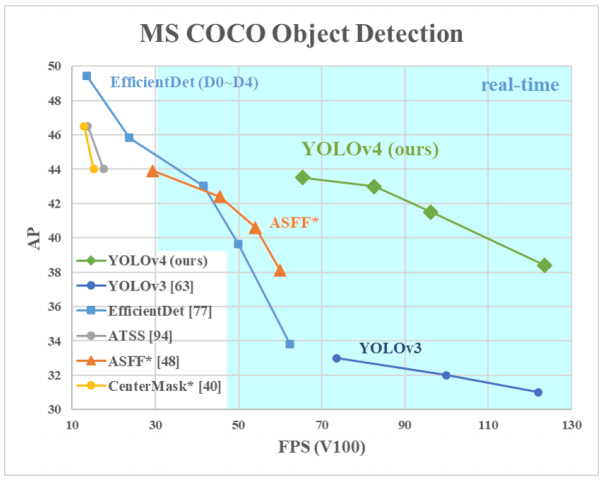
\includegraphics[width=1\textwidth]{NeuralNetwork/YOLO}
		\caption{The YOLO system} 
		\label{YOLO}
	\end{center}
\end{figure}

The network architecture of YOLO is based on GoogLeNet. It consists of 24 convolutional layers followed by two fully networked layers. The first 20 convolutional layers are pre-trained with the ImageNet dataset over a period of one week. The images in ImageNet have a resolution of 224 $\times$ 224, the final YOLO network takes images with a resolution of 448 $\times$ 448 as input. Also, the training always takes place with the entire images, without prior subdivision. \cite{Redmon.08.06.2015}\\

The advantage of YOLO lies primarily in its speed, which allows a video stream to be processed with a latency of less than 25 ms. This makes YOLO 1000 $\times$ faster than R-\ac{cnn} and 100 $\times$ faster than Fast R-\ac{cnn}. Since the entire image is presented to the network and not just individual parts of it, contextual information can be taken into account. For example, fewer errors due to interpretation of parts of the background as objects occur less frequently than with other systems. In addition, what is learned by the system can be better transferred to other areas, so that objects learned from photographs, for example, can also be recognised better in artistic representations than with other systems.  \cite{Redmon.08.06.2015} \cite{Redmon.17.02.2021}

The YOLO code as well as the code used for the training are open source.
